\documentclass[a4paper, 10pt]{article}
\usepackage{helvet}
\renewcommand{\familydefault}{\sfdefault}
\usepackage{pgf}
\usepackage{eurosym}
\usepackage{graphicx}
\usepackage{wasysym}
\usepackage{hyperref}
\usepackage{listings}
\usepackage{pxfonts}
\usepackage{verbatim}
\usepackage{color}
\usepackage{xcolor}
\usepackage{wrapfig}
\usepackage{enumitem}
\usepackage{booktabs}
\usepackage{gensymb}
\usepackage{tabularx}
\usepackage{currfile}

\hypersetup{
    bookmarks=true,         % show bookmarks bar?
    unicode=true,          % non-Latin characters in Acrobat’s bookmarks
    pdftoolbar=true,        % show Acrobat’s toolbar?
    pdfmenubar=true,        % show Acrobat’s menu?
    pdffitwindow=true,     % window fit to page when opened
    pdftitle={Assessments},    % title
    pdfauthor={Paul Vesey},     % author
    pdfsubject={Building Information Modelling },   % subject of the document
    pdfcreator={},   % creator of the document
    pdfproducer={xelatex}, % producer of the document
    pdfkeywords={'Graphics' }, % list of keywords
    pdfnewwindow=true,      % links in new PDF window
    colorlinks=true,       % false: boxed links; true: colored links
    linkcolor=violet,          % color of internal links (change box color with linkbordercolor)
    citecolor=magenta,        % color of links to bibliography
    filecolor=red,      % color of file links
    urlcolor=blue           % color of external links
}

\setlength\parindent{0pt}
\begin{document}

\lstset{language=HTML,
				basicstyle=\small,
				breaklines=true,
        numbers=left,
        numberstyle=\tiny,
        showstringspaces=false,
        aboveskip=-20pt,
        frame=leftline
        }
				
\begin{figure}
	\centering
	
\includegraphics[width=0.5\linewidth]{./Assignments/img/LITlogo}
\end{figure}


\begin{tabularx}{\textwidth}{ |l|X| }
	\hline
	\textbf{Subject:} & Revit MEP\\
	\textbf{Course:} & Building Information Modelling with Revit MEP\\
	\textbf{Session:} & Autumn 2021\\
	\textbf{Lecturer:} & Paul Vesey \footnotesize{BEng, MIE, HDip}\\
	\textbf{Filename:} & \currfilebase\\
	\hline
\end{tabularx}



\vspace{0.25cm}	
	
\part*{Assignment 1 (35\%) - Detached 2 Storey Residence}

\begin{tabularx}{\textwidth}{ |X|X| }
	\hline
	\textbf{Issue Date:} & 13-Feb-24 \\
	\hline 
	\textbf{Submission Date:}  & 9-March=24 \\
	\hline
\end{tabularx}


\section*{Assignment Outline}

This assignment will examine the following learning outcomes:\\

\begin{tabularx}{\textwidth}{ |c|X|c| }
	\hline
	\textbf{No.} & \textbf{Learning Outcome} & \textbf{Assessed} \\
	\hline 
	1  & Produce multi-view, isometric, and oblique drawings & Yes \\
	2  & Produce plan views; elevations, and sections of small to medium sized buildings. & Yes \\
	3  & Edit existing CAD drawings & Yes \\
	4  & Produce Revit generated material schedules and take-off lists & Yes \\
	5  & Use Revit to create presentation graphics and renderings & No \\
	\hline
\end{tabularx}


\vspace{1cm}

\begin{tabularx}{\textwidth}{ |l|X| }
	\hline 
	\textbf{Excellent (70+\%)} & Faithful recreation of the original drawings with no errors, and shows improvements over the original drawing set\\ 
	\hline
	\textbf{Good (56\% to 69\%)} & Recreation of the original drawing set with some minor errors or omissions in presentation and modelling \\
	\hline
	\textbf{Acceptable (40\% to 55\%)} & Recreation of the original drawing set with numerous minor errors or omissions in presentation and modelling that could be addressed with minimal additional work \\ 
	\hline
	\textbf{Poor ($<$40\%)} & Modelling incomplete, Views missing, Major Annotation Missing, general poor presentation of the design  \\
	\hline
\end{tabularx}

\vspace{1cm}




You are required to model a two storey house and to digitally submit you project file (.rvt) showing your model on one A4 sheet and four A1 sheets.


\newpage
\section*{Your Submission should contain the following drawings}



\begin{tabularx}{\textwidth}{ |c|c|X| }
	\hline
	\textbf{Sheet Size} & \textbf{Sheet No.} & \textbf{Title} \\
	\hline 
	A4  & AR-0001 & Cover Sheet \\
	A1  & AR-0002 & Ground Floor Plans and Internal Views \\
	A1  & AR-0003 & Upper Floor Plans and Internal Views \\
	A1  & AR-0004 & Foundations \\
	A1  & AR-0005 & Elevations \\
	A1  & AR-0006 & Sections and Details \\
	A1  & AR-0007 & Room Usage \\
	\hline
\end{tabularx}

Details of the requirements for each drawing are given below:\\

\subsection*{AR-0001 - Cover Sheet}
\begin{itemize}
	\item Three Dimensional (Aerial View) of the model (scaled to suit the sheet size) Shaded
	\item A list of the drawings in the design pack
\end{itemize}


\subsection*{AR-0002 - Ground Floor Plans and Internal Views}
\begin{itemize}
	\item Ground Floor Plans @ 1:50 with dimensions, Room Titles and some fixed furniture
	\item Ground Floor 3D Section
	\item Door and Window Schedule
\end{itemize}


\subsection*{AR-0003 - Upper Floor Plans and Internal Views}
\begin{itemize}
	\item Upper Floor Plans @ 1:50 with dimensions, Room Titles and some fixed furniture
	\item Upper Floor 3D Section
	\item Door and Window Schedule
\end{itemize}


\subsection*{AR-0004 - Foundations}
\begin{itemize}
	\item Foundation Plan @ 1:50 with dimensions
	\item Detail of Foundation
	\item 3D View of Foundation Layout
\end{itemize}



\subsection*{AR-0005 - Elevations}
\begin{itemize}
	\item South Elevation @ 1:50
	\item North, East and West Elevations @ 1:100
	\item Window Legend
\end{itemize}

\subsection*{AR-0006 - Sections, Details and Schedules}
\begin{itemize}
	\item Section thro' Kitchen / Sitting Room facing East @ 1:100
	\item Section thro' Kitchen / Sitting Room facing West (towards kitchen units) @ 1:100
	\item Section thro' the Hallway / Landing showing the Stairs @ 1:100
	\item One full height detail (Call-outs) @ 1:25, including Repeating Details showing the following:
	\begin{itemize}
		\item Foundation / External Wall / Floor Interfaces
		\item Facia / Soffit and Roof Details
		\item All necessary notes
	\end{itemize} 
\end{itemize}

\subsection*{AR-0007 - Room Usage}
\begin{itemize}
	\item Ground Floor Room usage Color Fill Legend @ 1:50
	\item First Floor Room usage Color Fill Legend @ 1:50
	\item Two Rendered Views (Cloud Render or Revit Local Render)
\end{itemize}


Additional Sheets may be submitted if so desired.

\newpage
\begin{flushleft}
\section*{Presentation and Submission}
\end{flushleft}


\begin{enumerate}
	\item All drawing sheets must have the TUS logo and be clearly marked 'Educational Exercise - Not for Construction'.  Titleblocks have been provided
	\item You are required to submit you project as a single Revit (.rvt) file through MS Teams
	\item Drawings should show all necessary information to communicate design intent
	\item The Revit filename should be of the form used in NA-2021 to I.S. EN ISO 19650-2-2018.  In this case, it will \textit{CADD06021-01-X-X-XXX-M3-\#\#\#-AR-0001-P9-D-0}, where \#\#\# is replaced by the last 3 digits of your K-number. An example would be \textbf{'CADD06021-01-X-X-XXX-M3-920-AR-0001-P9-D-0'}, for K-number K20001920.  Do not use spaces in the filename
\end{enumerate}


\newpage

\section*{Design Specification}



The total floor area of the house should be approx 150$m^2$\\

The following design may be used as a guide.  You may modify the proportions provided you maintain a protrusion at the front of the building.

\subsection*{Ground Floor}
\begin{itemize}
	\item Entrance Hall (2400mm wide)
	\item Universally Accessible Bathroom / Toilet
	\item Kitchen / Dining (with fixed and loose furniture)
	\item Living Room / Sitting Room (with direct access to kitchen)
	\item Ground Floor Bedroom (Playroom / Study)
	\item Externally accessed boiler house/shed
	\item Stairs 900mm wide (Rise 171.9mm, Going 280mm)
\end{itemize}



\begin{figure}
	\centering
	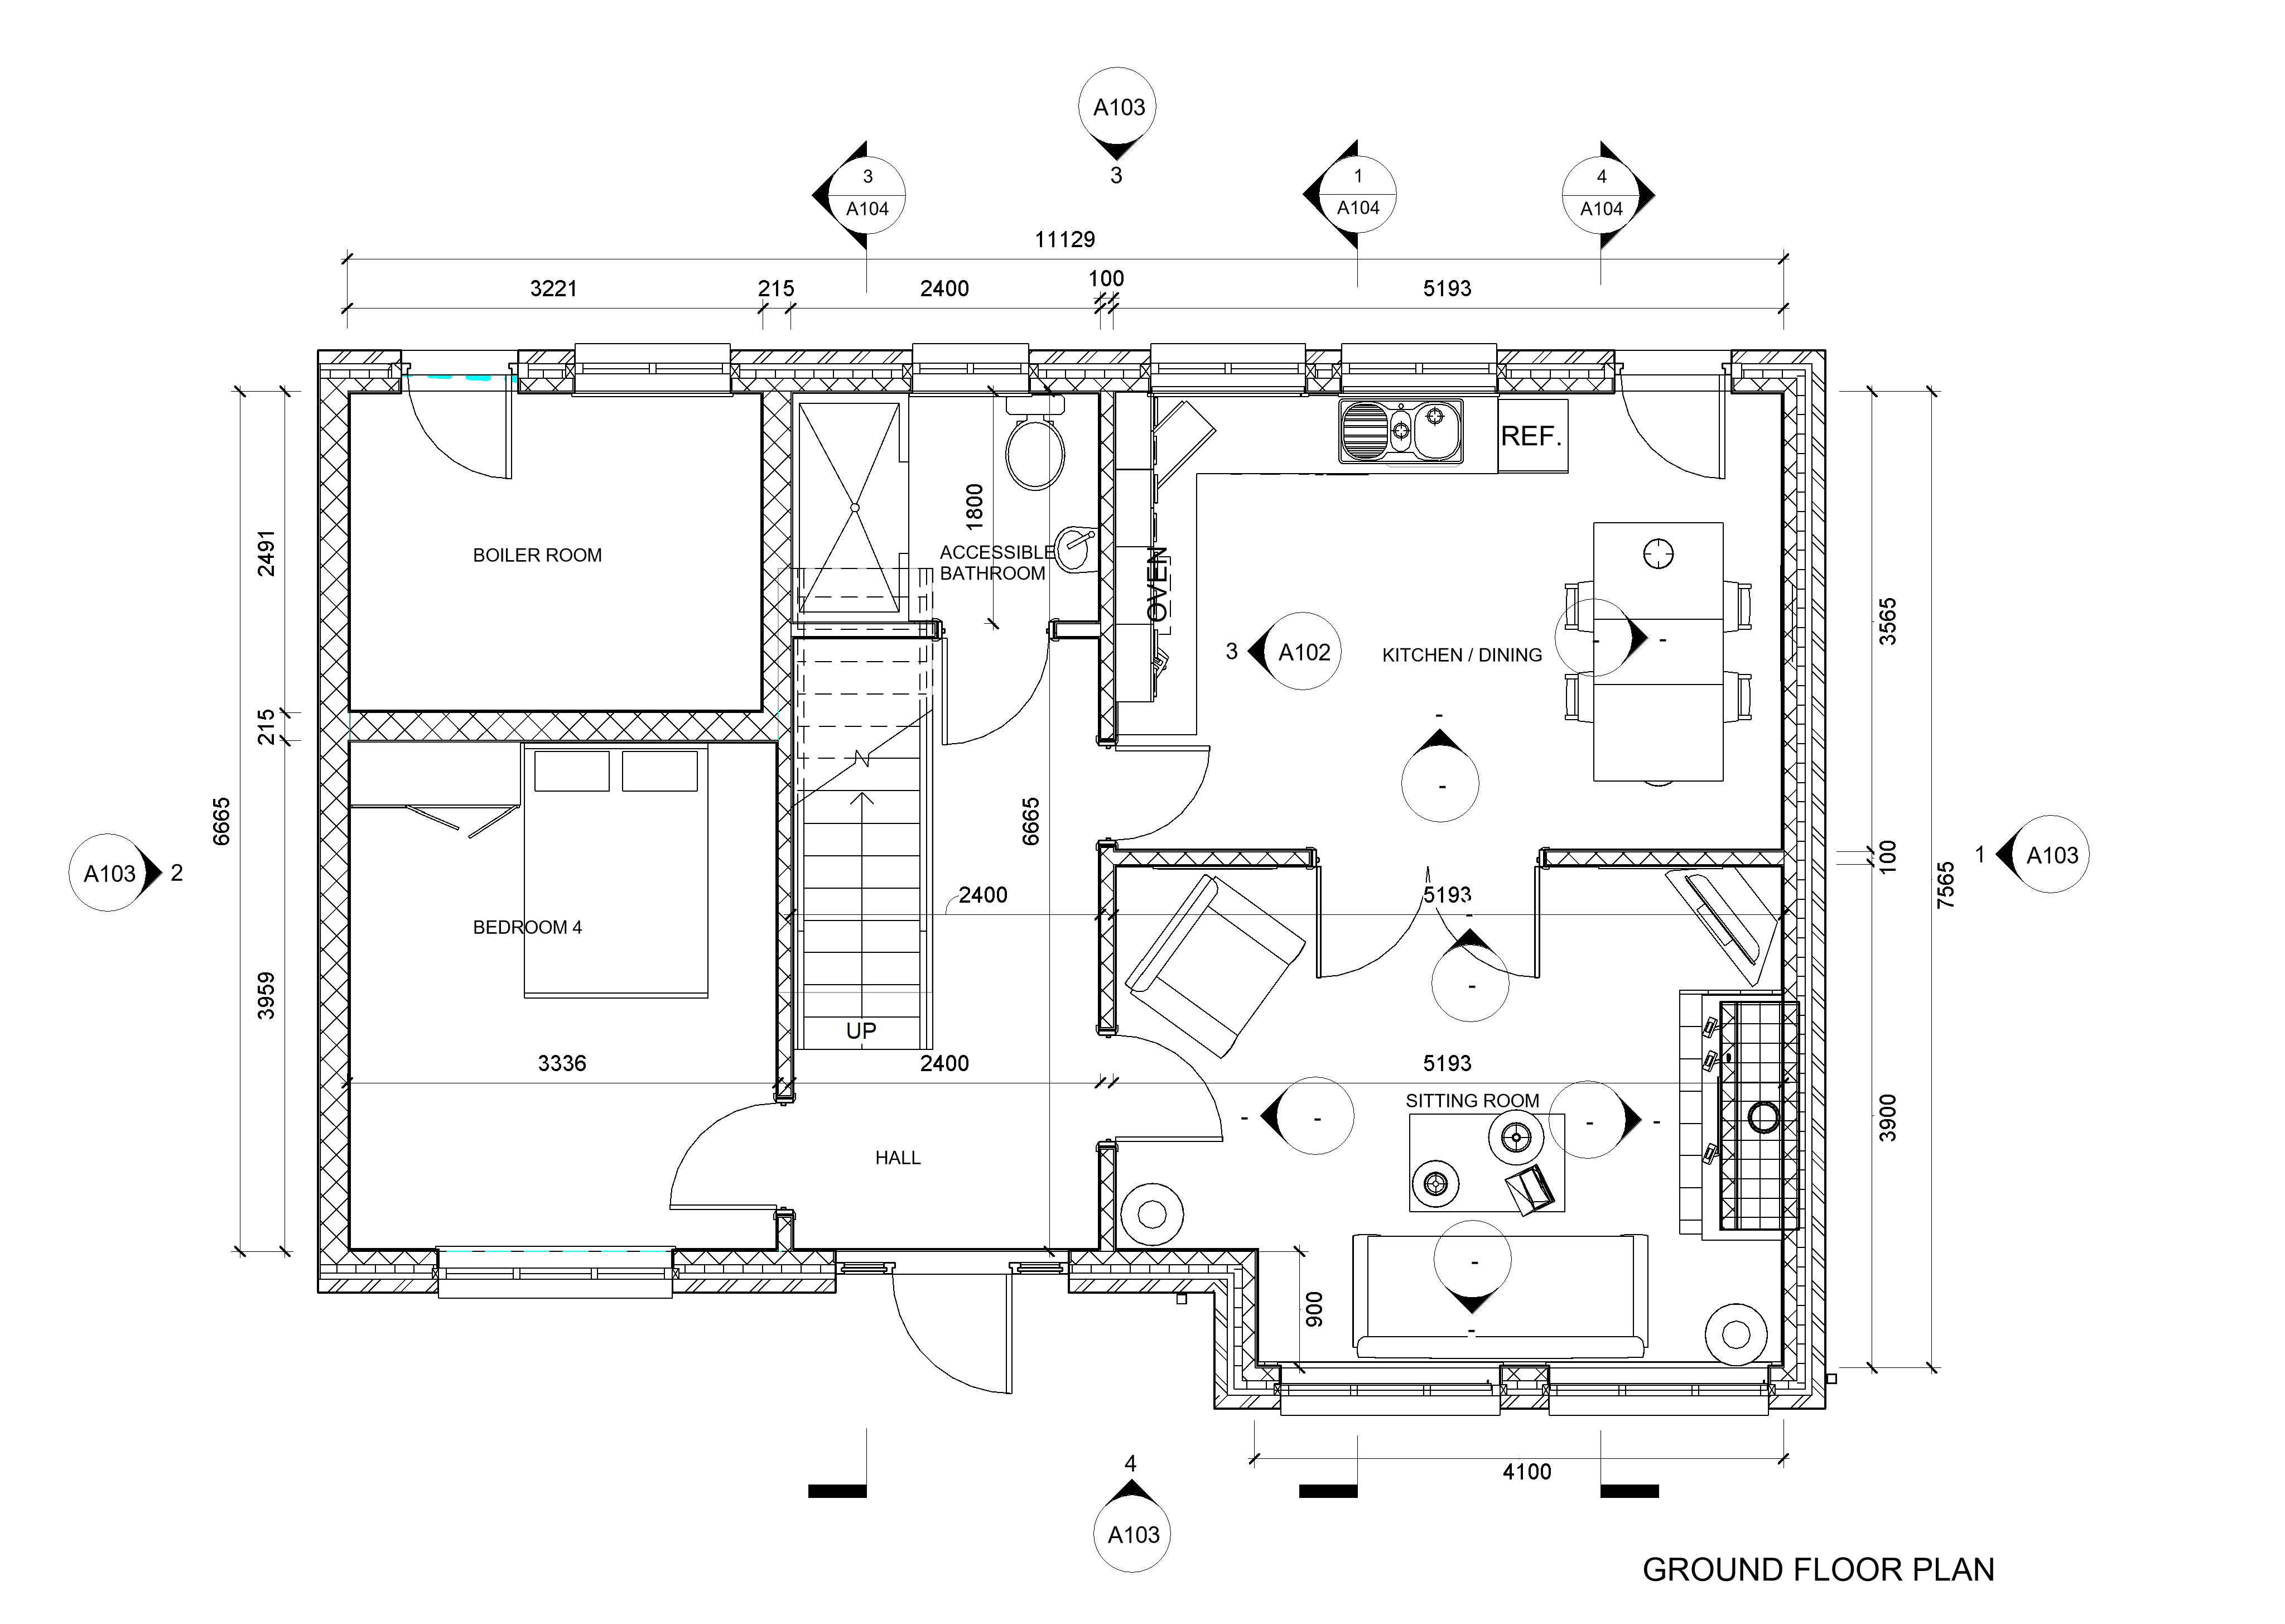
\includegraphics[width=1.0\linewidth]{./img/P01GroundFloorLevel.jpg}
	\caption{Ground Floor}
	\label{fig:p01groundfloorlevel}
\end{figure}


\newpage
\subsection*{Upper Floor Floor}
\begin{itemize}
	\item 3 Bedrooms with en-suite sanitary facilities
	\item Main Bathroom with Bath or Shower, WC and sink
	\item Hot Press
\end{itemize}



\begin{figure}[th]
	\centering
	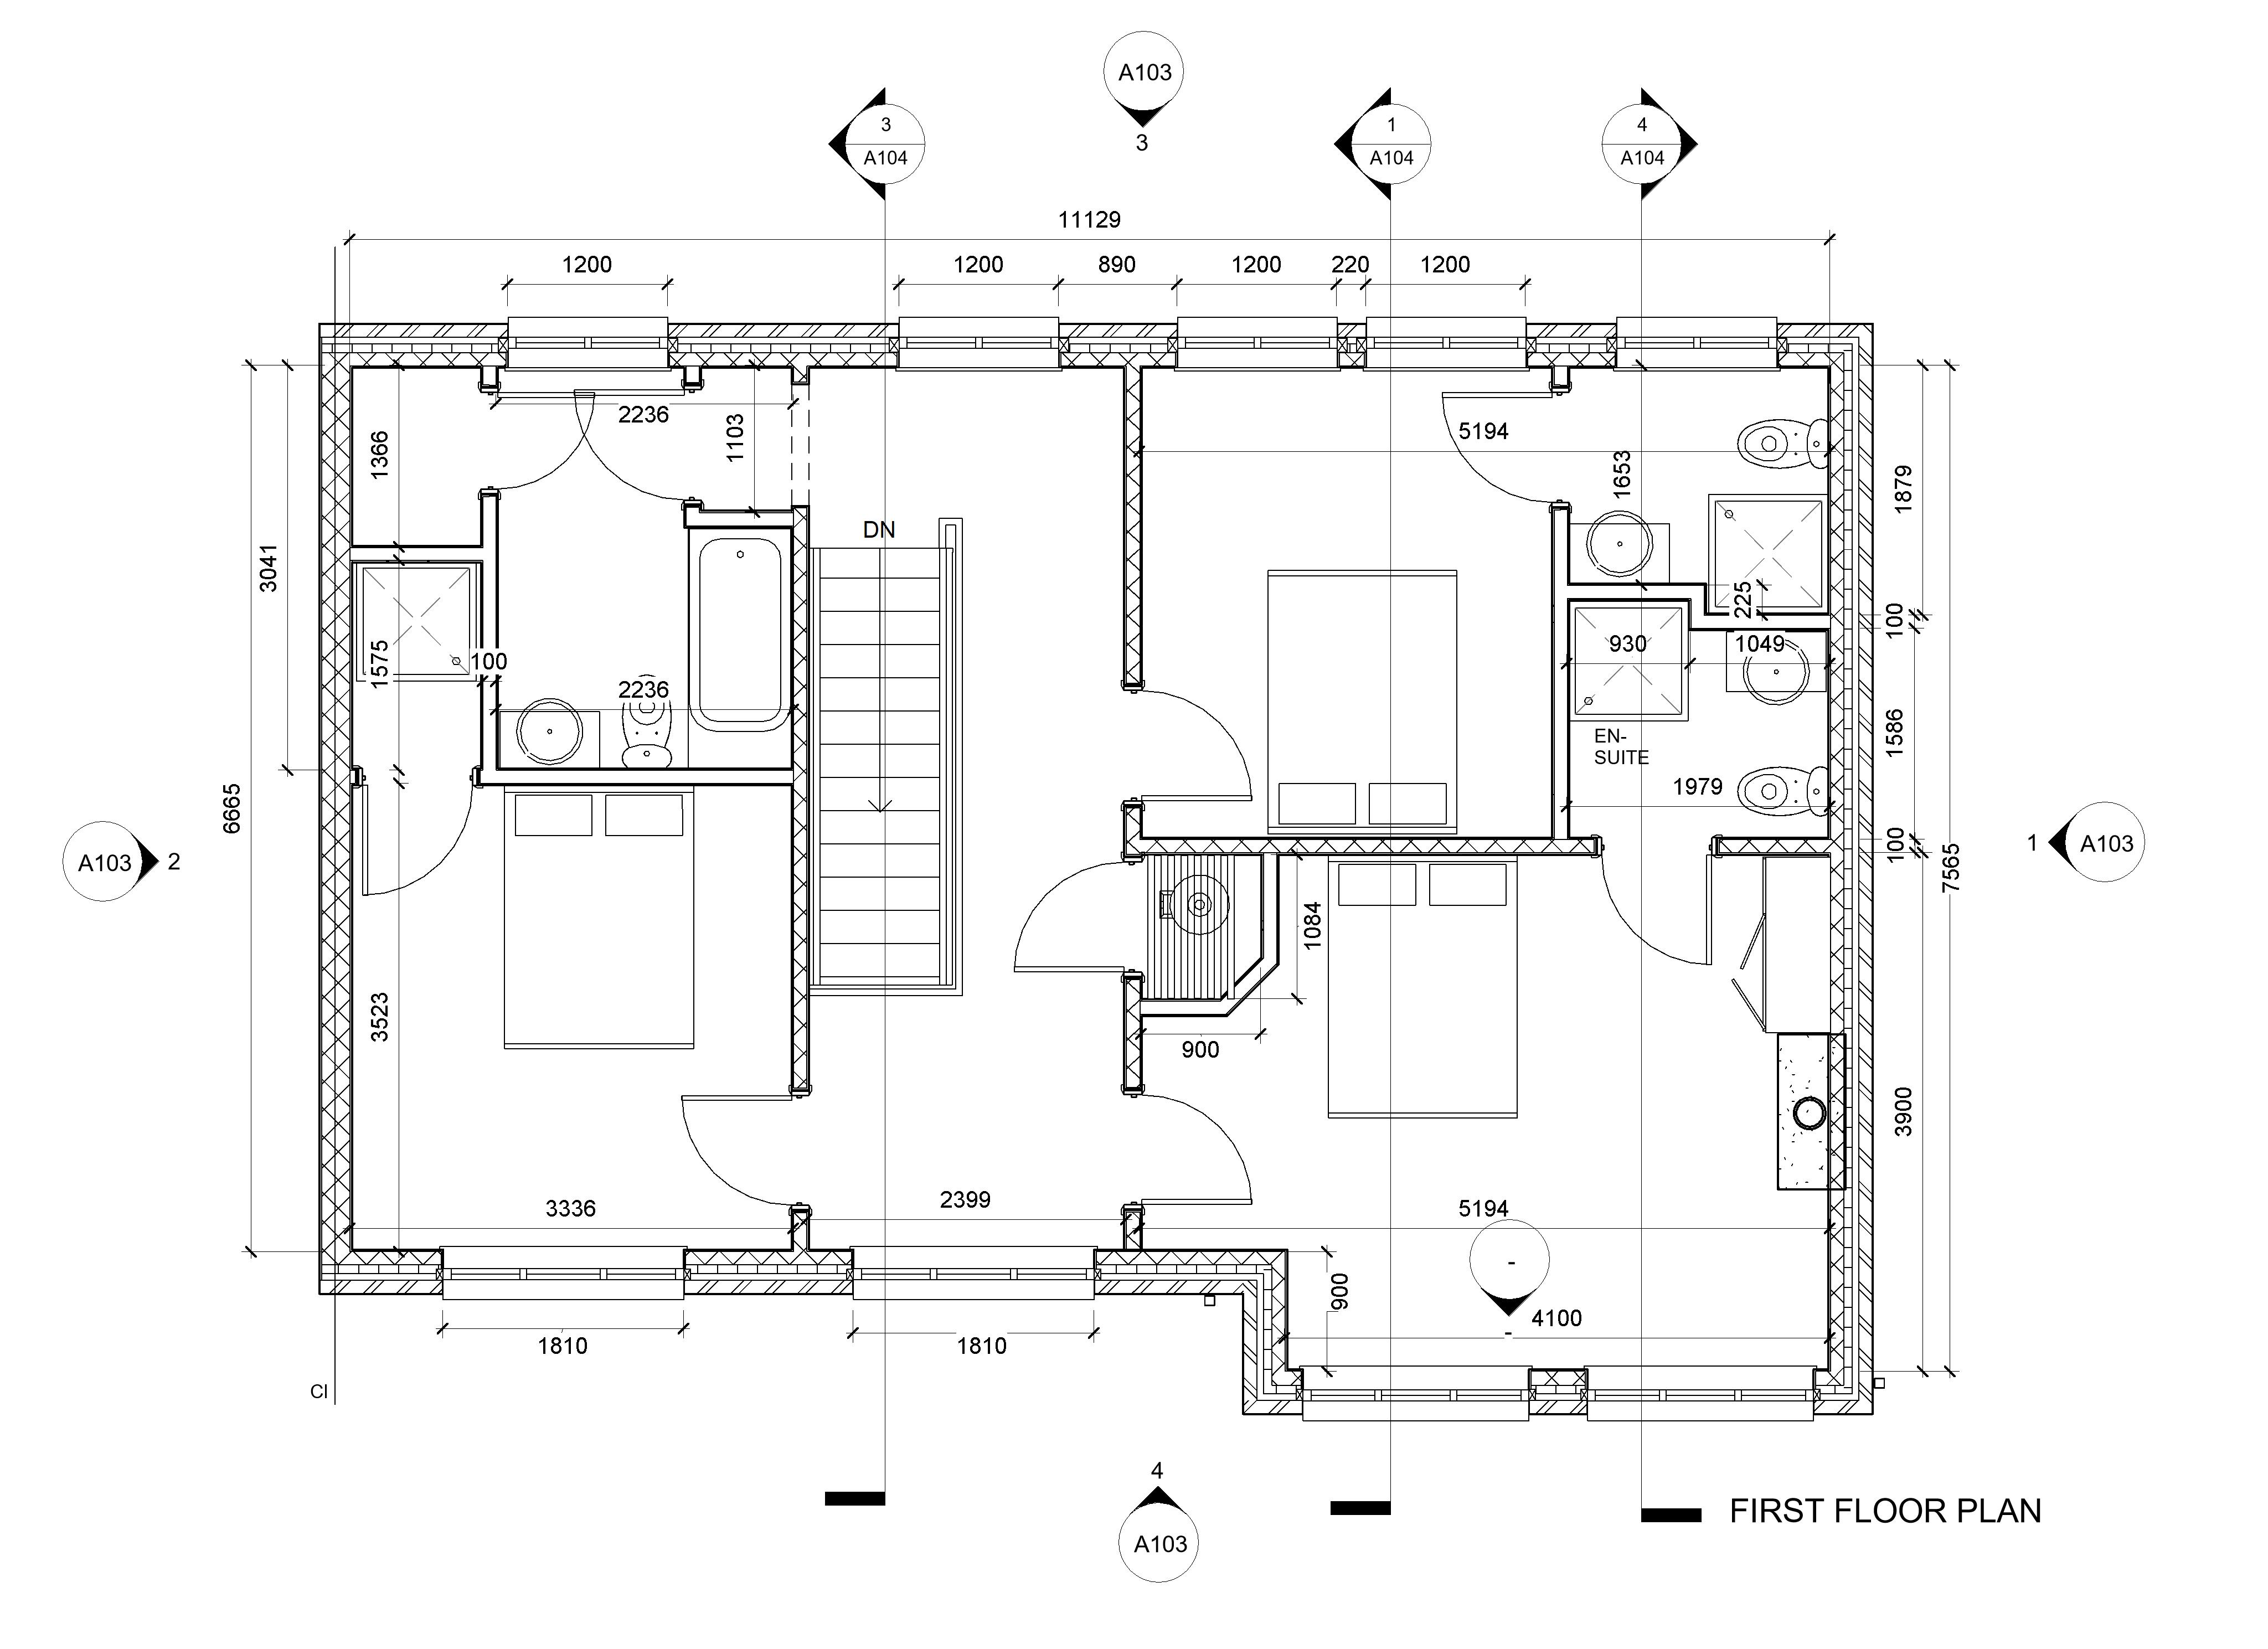
\includegraphics[width=1.0\linewidth]{./img/P01FirstFloorLevel.jpg}
	\caption{First Floor Plan}
	\label{fig:p01firstfloorlevel}
\end{figure}


\newpage
\section*{Construction Specification}


\textbf{External Wall Specification} 

External walls are to be twin leaf cavity construction.

\begin{enumerate}
	\item EF\_25\_10\_25\_Wall-Ext-Cav\_102Bwk-50Air-65Ins 100DBlk-15Rnd\&P
	\begin{itemize}
		\item 332mm wide insulated Cavity Walls over DPC level - Generally
		\item Made up of 102.5mm Brick / 50mm Air-gap / 65mm Insulation / 100mm Blockwork inner leaf
		\item Internal Finish 15mm (total) Render and Plaster
	\end{itemize}
	
	\item EF\_25\_10\_25\_Wall-Ext-Cav\_20Rnd-100Blk-50Air-65Ins-100DBlk-25Ins
	\begin{itemize}
		\item 360mm wide insulated Cavity Wall - not used
		\item 20mm Cement Render (Plinth) / 100mm block / 50mm Air-gap / 65mm Insulation / 100mm Block
		\item 25mm thick perimeter insulation up-stand to internal face
	\end{itemize}
	
	
	\item EF\_25\_10\_25\_Wall-Ext-Cav\_100Blk-115Conc-100Blk
	\begin{itemize}
		\item 315mm wide un-insulated Rising Wall
		\item 100mm Block / 115mm wide Concrete filled cavity / 100mm Block inner leaf
	\end{itemize}
	
	
	EF\_20\_05\_Wall-Fnd\_440DBlk (Trench Blockwork)
	\begin{itemize}
		\item 440mm wide Solid Trench Blockwork
	\end{itemize}

	EF\_25\_10\_25\_Wall\_225DBlk (Block on Flat)
	\begin{itemize}
		\item 245mm wide Blockwork
		\item 15mm Render and Plaster / 215mm Blockwork / 15mm Render and Plaster
	\end{itemize}

\end{enumerate}

\textbf{Foundations (Footings)}

\begin{itemize}
	\item 910 wide x 350 deep strip foundation
	\item Top of Strip foundation to be 900mm below Gr. Floor level
\end{itemize}



\subsection*{Internal Wall Specification}

\begin{itemize}
	\item Ground Floor Internal Walls
		\begin{itemize}
			\item Generally, Single leaf 100mm concrete block walls 15mm render / plaster both sides, (Wall-Part\_15Rnd\&P-100Blk-15Rnd\&P)
		\end{itemize}
	\item First Floor Internal Walls
		\begin{itemize}
			\item Landing Area: Single leaf 100mm concrete block walls, 15mm render / plaster both sides (Wall-Part\_15Rnd\&P-100Blk-15Rnd\&P)
			\item Elsewhere: 100mm timber stud partition, 15mm plaster slab / plaster both sides (Wall-Stud-Part\_15Gwb\&P-100Stud-15Gwb\&P) 
		\end{itemize} 
\end{itemize}



\subsection*{Floor Specification}


\begin{itemize}
	\item Ground Floor: Revit Library modified floor type (Floor-Grnd-Bearing) to be duplicated and used(Floor-Grnd-Bearing\_65Scr-100Ins-150Conc-DPM-50SBld-200Hcore)
	\begin{itemize}
		\item 65mm Sand \& Cement Screed on
		\item 100mm Floor Insulation on
		\item 150mm Reinforced Concrete Slab on
		\item Damp Proof Membrane on
		\item 50mm Sand Blinding on 
		\item 200mm Selected and Graded Hardcore laid in 2 No. 100mm layers
	\end{itemize}
	\item First Floor: Revit Library modified floor type (Floor\_Timber\_25Cbd-225Joist) may be used: Finished First Floor Level to be 2750mm (GFL to FFL)

\end{itemize}












\subsection*{Windows and Doors}
\begin{itemize}
	\item Head height - 2100mm
	\item Revit Library standard door types may be used
	\item External Front Door: Decorative type (panelled door with glazed side panels)
	\item External Kitchen and Boiler house doors to have glazed panels
	\item Generally, internal single doors to be standard flush-panel or regency panelled type
	\item Kitchen to living room doors to be double leaf, glazed multi-panel style
	\item Windows generally to be double or triple sash type with opening vents
\end{itemize}


\subsection*{Electrical Fittings -- Optional: no marks allocated}
\begin{itemize}
	\item Kitchen and Living Room only, to be visible in Section or Camera View
	\item 2 No. Ceiling or Wall mounted light fittings per room
	\item 2 no. Twin Switched Socket power outlets per room
\end{itemize}


\subsection*{Ceilings}
\begin{itemize}
	\item 3mm Skim Coat Plaster on Gypsum Wall Board
	\item Revit Library 'modified' ceiling type (Compound Ceiling Plain)
	\item Ceiling Cut-outs required for Stairs and Dormer Window.
\end{itemize}



\subsection*{Roof Type}
\begin{itemize}
	\item Roof by Footprint
	\item Pitch 35\degree
	\item Main Roof overhang to be approx 300mm clear of outer leaf	
\end{itemize}



\subsection*{Roof Construction Specification}
\begin{itemize}
	\item Revit roof type 'Roof\_Pitched\_38Tile-25Bat-0Felt-25Bat-100Ins-150Truss-12PBd to be modified as follows: Roof\_Pitched\_38Tile-38Bat-0Feld-150Truss.
	\begin{itemize}
		\item 38mm Roofing Tile on 
		\item 38mm battens on 
		\item Roof Membrane on 
		\item 150mm Structure (Truss / Rafter)
	\end{itemize}
\end{itemize}

\subsection*{General Building -- Optional: no marks allocated}
Provide the following
\begin{itemize}
	\item Facia Boards, Flat Soffits, Rainwater Gutters, Downpipes and all necessary information to communicate design intent.
\end{itemize}

\subsection*{Site}
\begin{itemize}
	\item A basic flat topographical layer (Toposurface) is to be inserted in the Site View.  The toposurface be created at an elevation of -225mm
\end{itemize}


\end{document}